\documentclass[wes, manuscript]{copernicus}

%% \usepackage commands included in the copernicus.cls:
%\usepackage[german, english]{babel}
%\usepackage{tabularx}
%\usepackage{cancel}
%\usepackage{multirow}
%\usepackage{supertabular}
%\usepackage{algorithmic}
%\usepackage{algorithm}
%\usepackage{amsthm}
%\usepackage{float}
%\usepackage{subfig}
%\usepackage{rotating}


\usepackage{tabularx}
\usepackage{mathtools}
\usepackage{mathrsfs}
\usepackage{amsmath}
%\usepackage[short]{optidef}
\usepackage{xcolor}
\usepackage{amsfonts}

% Colors
%---------------------------------------------------------------------------------
\definecolor{C1}{RGB}{31,119,180}
\definecolor{C2}{RGB}{255,127,14}
\definecolor{C3}{RGB}{44,160,44}
\definecolor{C4}{RGB}{214,39,40}

% Some  auxiliary commands for ease of mathematics notations
%---------------------------------------------------------------------------------
% Derivatives and differentials
\newcommand{\ds}{~\text{d}\boldsymbol{s}}
\newcommand{\dzeta}{~\text{d}\boldsymbol{\zeta}}
\newcommand{\pder}[2]{\frac{\partial #1}{\partial #2}}
\newcommand{\bs}[1]{\boldsymbol{#1}}
\newcommand{\dx}{\text{d}\boldsymbol{x}}
\newcommand{\dt}{\text{d}t}
\newcommand{\ddt}[1]{\frac{\text{d} #1}{\text{d} t}}
% Integrals
\newcommand{\stint}{\int_{0}^{T} \int_{\Omega}}
\newcommand{\sint}{\int_{\Omega}}
\newcommand{\Tint}{\int_{0}^{T}}
\newcommand{\tint}{\int_{0}^{t}}
% Filtered variables
\newcommand{\utilde}{\widetilde{\bs{u}}}
\newcommand{\ptilde}{\widetilde{p}}
\newcommand{\ctnhat}[1]{\widehat{C}_{T,#1}'}
\newcommand{\ctihat}{\widehat{C}_{T,i}'}
\newcommand{\cthat}{\widehat{C}_T'}
% Other symbols
\newcommand{\ctmax}{C_{T,\text{max}}'}
\newcommand{\cti}{C_{T,i}'}
\newcommand{\ctn}[1]{C_{T,#1}'}
\newcommand{\R}{\mathscr{R}}
\newcommand{\J}{\mathscr{J}}
\newcommand{\Jtilde}{\tilde{\mathscr{J}}}
\newcommand{\Jgrad}{\nabla \Jtilde}
\newcommand{\Lagr}{\mathscr{L}}
\newcommand{\eperp}{\bs{e}_\perp}
\newcommand{\eperpi}{\bs{e}_{\perp,i}}
\newcommand{\etransi}{\bs{e}_{\parallel,i}}
\newcommand{\ex}{\bs{e}_x}
\newcommand{\ey}{\bs{e}_y}
\newcommand{\ez}{\bs{e}_z}
\newcommand{\eperpn}[1]{\bs{e}_{\perp,#1}}
\newcommand{\vi}{\frac{1}{A_i} \sint \R_i (\bs{s})~\utilde \cdot \eperpi \ds}
% Operators
\newcommand{\innerproduct}[2]{\bigg( #1, #2 \bigg)}
\newcommand{\innerproductsmall}[2]{\big( #1, #2 \big)}
\newcommand{\sumturbines}{\sum_{i=1}^{N_t}}
\newcommand{\diracdelta}{{\delta}}
\DeclareMathOperator*{\argmin}{arg\,min}






\begin{document}

\title{Towards practical dynamic induction control of wind farms: analysis of optimal control dynamics and sinusoidal induction control of first-row turbines}
\runningtitle{Towards practical dynamic induction control of wind farms}

\Author[]{Wim}{Munters}
\Author[]{Johan}{Meyers}
\affil[]{Department of Mechanical Engineering, KU Leuven, Celestijnenlaan 300A, 3001 Leuven, Belgium}
\runningauthor{Munters and Meyers}
\correspondence{wim.munters@kuleuven.be}



\received{}
\pubdiscuss{} %% only important for two-stage journals
\revised{}
\accepted{}
\published{}

\firstpage{1}
\maketitle

\begin{abstract}
	Wake interactions between wind turbines in wind farms entail reduced energy extraction in downstream rows, inciting research into coordinated wind-farm control strategies for optimal power extraction. In recent work, optimization and large-eddy simulation were combined to study optimal dynamic induction control of wind farms with power gains up to 20\% (Munters \& Meyers 2017 \emph{Phil Trans R Soc A} \textbf{375}, 20160100, doi:10.1098/rsta.2016.0100). However, computational costs associated with the optimal control simulations impede practical implementation of this work. Furthermore, the resulting optimal control signals are tuned to specific flow events and hence cannot be used in practice, and the complexity of these signals complicated the derivation of simplified control strategies. The current work focuses on further analysis of the optimization results of Munters \& Meyers. The analysis shows that wind-farm controls are optimized in a uni-directional manner with little upstream propagation of information, and that turbines can be classified into first-row, intermediate-row, and last-row turbines based on their optimal control dynamics. Furthermore, it is found that optimally-controlled first-row turbines periodically shed vortex rings leading to enhanced wake mixing. This behavior is mimicked with a simple sinusoidal thrust control strategy, resulting in robust power gains for turbines in the entrance region of the farm.
\end{abstract}


\copyrightstatement{TEXT}


\introduction  %% \introduction[modified heading if necessary]
Wake interactions between turbines within a wind farm cause reduced power extraction and increased turbine loading in downstream rows. The current control paradigm in such farms optimizes performance at the wind-turbine level and does not account for these interactions, resulting in sub-optimal wind-farm efficiency. In contrast, control strategies at the farm level allow to influence wake interactions and promise to improve overall wind-farm performance by improving wind conditions for downstream turbines, i.e. by redirecting propagating wakes (yaw control, see e.g. \citealp{fleming2014evaluating, gebraad2016wind, campagnolo2016wind}) or by affecting the induced wake velocity deficits (axial induction control, see e.g. \citealp{nilsson2015large, annoni2016analysis, bartl2016experimental}). A more exhaustive survey of wind-farm control in a broader context can be found in \cite{knudsen2015survey} and \cite{boersma2017tutorial}. 

In contrast to the studies cited above, which focus on static setpoint control of wind farms, \cite{goit2015optimal} introduced a dynamic induction control approach based on large-eddy simulations and adjoint gradient optimization. The methodology was applied to the asymptotic case of a fully-developed `infinite' aligned wind farm, and power gains of about 16\% were quantified. Later, this approach was also used in induction control studies of wind farms with entrance effects in \cite{goit2016optimal} and, more recently, in \cite{munters2017optimal}, where similar gains in the order of 15\%--20\% were achieved. 
It is important to note that the computational cost of this dynamic induction control methodology is orders of magnitude too high for direct implementation, and the complex optimal control signals generated by the simulations are highly tuned to specific flow events and cannot be translated to practical flow conditions. However, the methodology allows to assess the theoretical potential for wind-farm control, and an increased understanding of the flow physics of controlled wind farms could lead to simplified control strategies that could be applied in practice.  

Very recently, the methodology of \cite{goit2015optimal} was generalized to include dynamic yaw control in \cite{munters2018dynamic}. In this study, induction control and yaw control were compared for a relatively small aligned wind farm, and yaw control was found to yield higher power gains for this setup. Furthermore, the high potential of combined induction and yaw control was quantified, and analysis of the yaw control signals allowed to identify practical simplified dynamic yaw control strategies. The search for similar practical control strategies for yaw control has remained unsuccessful to date. 

The current paper presents efforts on understanding optimal control dynamics and identifying the flow mechanisms behind the power increase observed in the optimal induction control simulations in \cite{munters2017optimal} (further denoted as MM17), with the aim of harnessing them in tractable dynamic induction wind-farm controllers. The analysis presented here will lead to the identification of a coherent flow mechanism in the wake of optimally controlled first-row turbines, responsible for part of the power increase in the optimal control simulations. This resulted in a new derived simplified dynamic axial induction control strategy for first-row turbines producing a robust power increase in the second row, irrespective of precise local flow details. However, it will be shown that the controls responsible for the remainder of the power gains in the optimal control simulations are tuned to specific flow conditions. This complicates the analysis of downstream rows, and has thus far impeded the derivation of similar control strategies for the latter.

The outline of the paper is as follows: first, Section~\ref{sec:optimal_control_sims} discusses the numerical setup and optimal control simulations of MM17 that will be further analysed in the current paper. Section~\ref{sec:analysis_controls_analysis} presents an analysis of the control and thrust force dynamics, and performs some numerical experiments to elucidate characteristics of the optimal controls. It will be shown that the coherent behavior of turbines situated in the first row of the wind farm stands out from their downstream counterparts. Hereafter, Section~\ref{sec:analysis_flow_vis} identifies the shedding of vortex rings from the first row based on a flow visualization. Further, a simple sinusoidal thrust control approach is presented that successfully mimics this process with a robust increase in power extraction extraction in the second row. Next, Section~\ref{sec:analysis_intermediate} shortly discusses the behavior of the intermediate rows, i.e. turbines which have both upstream and downstream neighbors, for which similar simple control strategies have not been identified thus far. In conclusion, Section~\ref{sec:analysis_summ} summarizes the main findings of this paper.

\section{Description of optimal control simulations}\label{sec:optimal_control_sims}
The current section describes the optimal control simulations performed by Munters \& Meyers \cite{munters2017optimal}, of which the results are further analyzed in the current paper. First, the methodology and numerical setup is detailed. Afterwards, the simulation results are discussed. 

\subsection{Methodology \& numerical setup}

\begin{figure}
	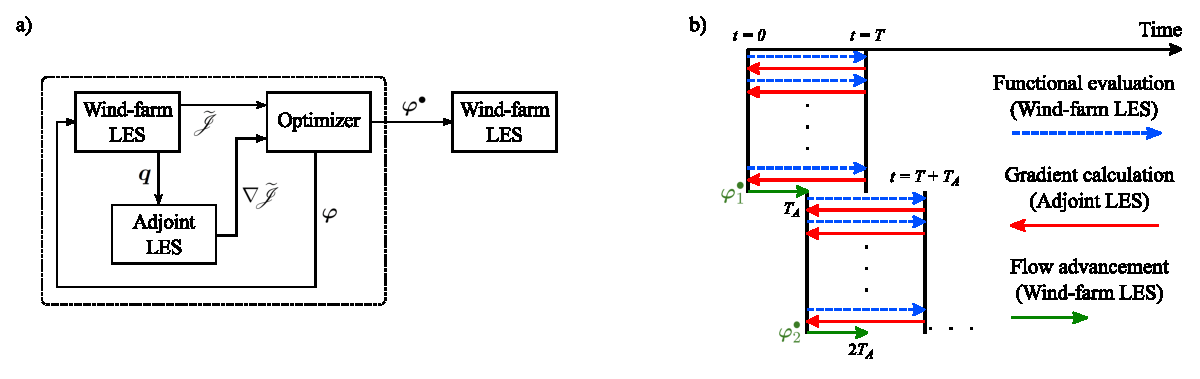
\includegraphics[width=\textwidth]{figure1.eps}
	\caption{Schematic overview of wind-farm optimal control methodology from MM17. \emph{a)} Control block diagram with adjoint gradient-based optimization and LES flow models illustrating data flow of (optimal) controls $\bs{\varphi}^{(\bullet)}$, system state $\bs{q}$, cost functional $\J$ and its gradient $\nabla \J$. \emph{b)} Receding horizon framework subdividing time into discrete flow advancement windows of length $T_A$ with prediction horizon $T$. Each arrow represents a forward or adjoint LES. Every window consists of an optimization stage (blue and red lines) follow by a flow advancement stage with optimal controls $\bs{\varphi}^{\bullet}$ (green lines).  \label{fig:optimization_meth}}
\end{figure}

Throughout the analysis, the focus will lie on the overinductive fast-response case C3t5, as it was observed to exhibit similar flow statistics as the maximum yield case C3t0, but with smoother thrust force dynamics.

Optimal control based on LES and optimization

Receding-horizon framework (maak 1 gecombineerde figuur)

Optimal control problem

\begin{alignat}{4}
& \underset{\bs{\varphi}, \bs{q}}{\text{minimize}}  & \qquad  \J(\bs{\varphi}, \bs{q}) &= - \Tint \sum_{i=1}^{N_t} P_i ~\dt  & \label{eq:costfunction}\\
& \text{s.t.}                      			&         \frac{\partial \utilde}{\partial t} + \big(\utilde \cdot \nabla \big)~ \utilde &= - \nabla (\ptilde + \ptilde_\infty) / \rho - \nabla \cdot \boldsymbol{\tau}_{sgs} + \sum_{i=1}^{N_t} \bs{f}_i \qquad  & \text{in } \Omega \times (0,T], \label{eq:NSmomentum_constraint} \\
&                                                   &        \nabla \cdot \utilde&=0 									        & \text{in } \Omega \times (0,T], \label{eq:NScontinuity_constraint}\\
&                                                   &        \tau \ddt{\ctihat}&=\cti - \ctihat 								& i=1\dots N_t~\text{in } (0,T],  \label{eq:ctihat_constraint}\\
&                                                   &        C_{T,\text{min}}' \leq~ &\cti \leq C_{T,\text{max}}'				& i=1\dots N_t~\text{in } (0,T],  \label{eq:boxct_constraint}
\end{alignat}
Define turbine forces and powers!

Focus on C3t5 case.

${\J} \nabla\J \bs{\varphi}^{\bullet}$

\subsection{Simulation results}

\section{Thrust coefficient analysis and numerical experiments}\label{sec:analysis_controls_analysis}

The current section focuses on the optimal thrust coefficients generated by the optimal control simulations in MM17, and performs numerical experiments to uncover some of the characteristics of these controls and their dependence on the local flow conditions. 

First, the thrust coefficient signals themselves are analyzed in Section~\ref{sec:analysis_controls_analysis}. Second, the optimized thrust coefficients are applied only to subsets of turbine rows in Section~\ref{sec:application_subset}. In this way, the interdependency of optimized thrust coefficients in different rows can be evaluated. Third, additional optimal control simulations, in which only one single active row is optimized, are discussed in Section~\ref{sec:optimization_single}. These optimizations provide an indication on how increased power potential is distributed among the rows, and allows to compare the resulting single-row optimized thrust coefficients with the fully cooperative coefficients from case C3t5. Fourth, Section~\ref{sec:modified_thrust} evaluates the dependency of optimized thrust coefficients on specific flow conditions. This is done by running test simulations in which the coefficients are modified to eliminate any possible correlations to specific flow events at given times. Finally, Section~\ref{sec:analysis_discussion} discusses the main conclusions from the abovementioned sections, and summarizes the lessons learned.

\subsection{Analysis of thrust coefficient signals}\label{sec:analysis_thrust}

Figure~\ref{fig:controls} illustrates the time evolution of some of  the thrust coefficients $\cthat$ in the C3t5 case. The figure illustrates that, for all rows but the last one (i.e. R12), $\cthat$ varies significantly in time, and that the amplitudes and frequencies of these variations are somewhat higher in the upstream rows of the farm. In contrast, row 12 features only minor unsteadiness at lower frequencies, and has an increased mean value of $\cthat$. This relatively steady behavior of the last row can be explained by the fact that there are no further downstream turbines that could benefit from row 12 actively influencing local flow conditions, hence the row optimizes its own power greedily. The increase in mean $\cthat$ can be explained based on Figure~\ref{fig:ct_sweep}, which illustrates the power extraction as a function of steady $\cthat$ for unwaked turbines, subject to identical turbulent inlet as in case C3t5. Although momentum theory predicts maximal power extraction for steady uniform inflow at $\cthat = 2$, the actual optimal steady value for the ADM at the current spatial resolution lies somewhat higher at $\cthat \approx 2.4$, for which power extraction is about 1.4\% higher than at $\cthat = 2$. This behavior is related to the overprediction in ADM power due to the diffuse turbine representation on typical simulation grids discussed in Section~\ref{sec:meth_adm}: the mass flow through the rotor disk at $\cthat > 2$ is slightly too high compared to momentum theory, resulting in a  shift of optimal $\cthat$ towards somewhat higher values. Although the linear fit $C_P' = a \cthat$ introduced in Appendix~\ref{ch:app_adm} eliminates the error in maximal power extraction, it does not correct the value of the optimal $\cthat$ (note that this could be achieved through a more complex relation between $C_P'$ and $\cthat$). Even though this explains the slight increase in mean $\cthat$ for greedily optimized last-row turbines, this does not undermine the overall power gains of the optimal control cases in MM17, which all feature power gains well over 10\%. Returning to the more complex thrust coefficients in the other rows it is worth noting that, based on the current dataset, no statistically significant correlations between thrust coefficients of different turbines could be found. Furthermore, attempts towards linking thrust coefficient dynamics to upstream flow measurements (e.g. velocities, shear or kinetic energy) through linear regression models and random forest regressors have been unsuccessful to date. 

\begin{figure}
	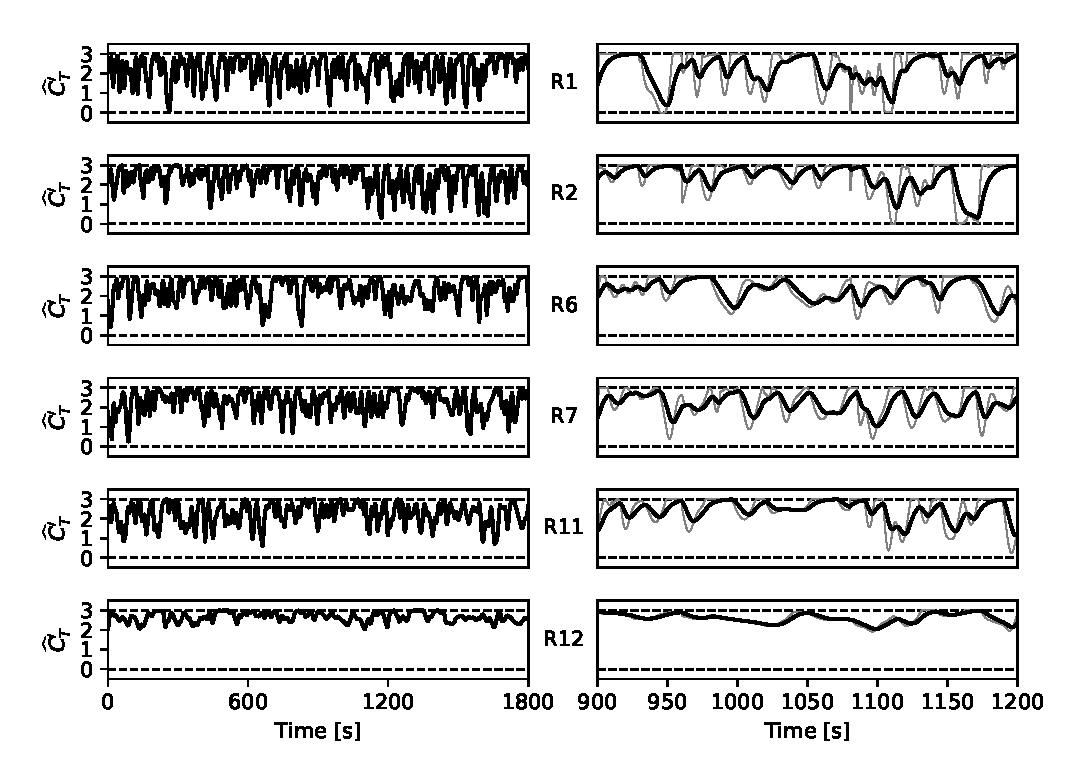
\includegraphics[width=\textwidth]{controls.eps}
	\caption{Time evolution of the thrust coefficient $\cthat$ for a selection of optimally controlled turbines  of case C3t5. \emph{Left: } Total time horizon. \emph{Right: } Zoomed view, including setpoint $C_T'$ in gray. \label{fig:controls}}
\end{figure}

\begin{figure}
	\includegraphics[width=\textwidth]{sweep_ct.eps}
	\caption{Normalized power extraction as a function of steady thrust coefficient $\cthat$ for wind turbines subject to the same freestream turbulent inflow as in case C3t5. Every dot corresponds to one LES.\label{fig:ct_sweep}}
\end{figure}

\begin{figure}
	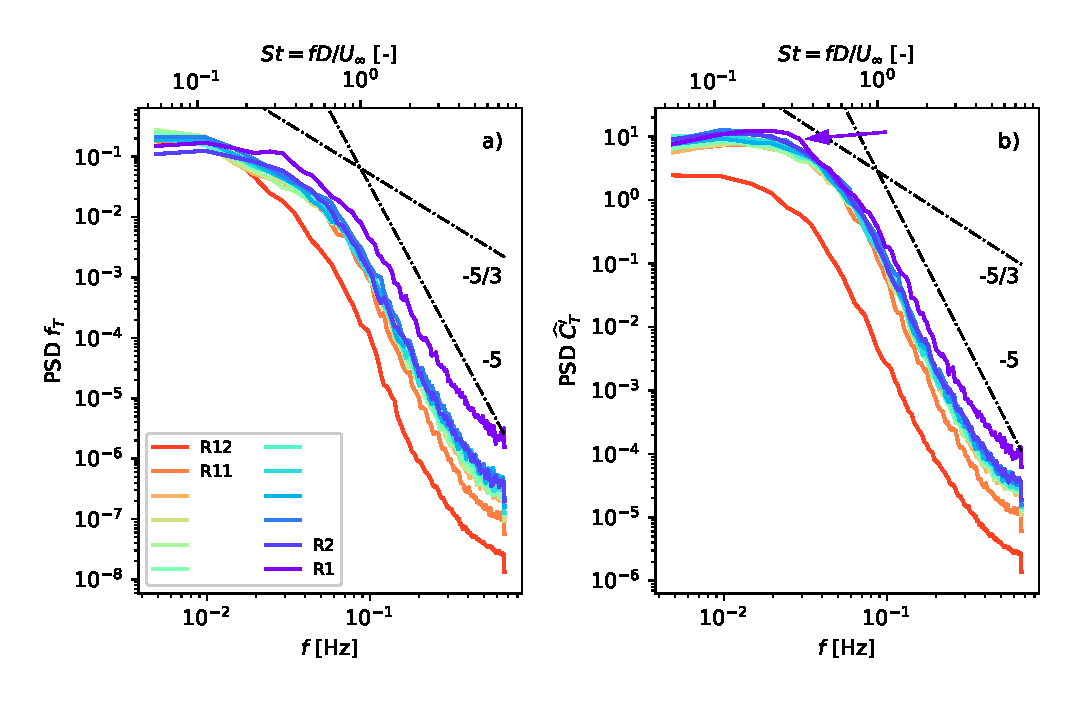
\includegraphics[width=\textwidth]{spectra_thrust_cthat.eps}
	\caption{Power spectral density (PSD) estimates of the row-averaged thrust force $f_T$ (\emph{a}) and thrust coefficient $\cthat$ (\emph{b}) as a function of frequency $f$ (bottom axis) and non-dimensional Strouhal number $St$ (top axis). \label{fig:spectra_thrust_cthat}}
\end{figure}

Figure~\ref{fig:spectra_thrust_cthat}a,b illustrate power spectral densities of the row-averaged thrust forces and thrust coefficients respectively. The figure illustrates that the variances of both the thrust coefficients and their resulting forces are highest in row 1. Further downstream, rows 2 to 11 have very similar spectral behavior, and row 12 shows significantly lower variability. The high-frequency slopes of around $-5$ observed both for $f_T$ and $\cthat$ indicate that force variability on short timescales is caused mainly by thrust coefficient variations, whereas the slower thrust force dynamics tend more to a $-5/3$ slope, suggesting that these are governed by the unsteadiness in the turbulence instead. Note that, even though the spectra for all rows except row 12 collapse at frequencies below $0.05$ Hz, the first-row spectrum shows a small yet significant peak at $f \approx 0.02 \dots 0.03$ Hz ($f D / U_\infty \approx 0.2 \dots 0.3$) as indicated by the purple arrow, which also translates to an increased spectral content of the first row thrust force at these frequencies. It will be shown later in this paper that variations in the thrust coefficient around this frequency can be harnessed to increase power extraction in the second row. 

\subsection{Application of optimal thrust coefficients to subsets of turbine rows}\label{sec:application_subset}

In order to further study how the optimal controls increase overall wind-farm power, Figure~\ref{fig:multirow} illustrates power extraction resulting from applying a subset of the optimal controls to specific turbine rows only. Figure~\ref{fig:multirow}a depicts simulation results for which the  optimized controls are applied \emph{only to one specific row}, with the thrust coefficient in all other rows kept at the reference value of $\cthat = 2$. From the figure it can be seen that only for the controls of the first row (R1) this results in a significant power increase in rows 2 and 3. This indicates that the optimal controls, as generated by the optimization at the wind-farm level, depend on the precise flow conditions caused by upstream control actions, and can hence only be applied independently for the first row, which has no upstream dependence by definition. 

Figure~\ref{fig:multirow}b shows results from simulations in which the controls are applied \emph{for all rows up to a certain row}, i.e. R1--R3 indicates the application of optimized controls generated by case C3t5 to rows 1, 2, and 3. An interesting observation from this figure is that , for any row $i$ except the last one, the power potential as observed in case C3t5 is almost fully recovered by only applying the optimal controls up to row $i-1$. This suggests that self-optimization is very limited: the optimal controls for a given turbine are designed to create favorable flow conditions in the downstream rows instead of increasing local power. Furthermore, although the discussion in the previous paragraph has shown that downstream controls are optimized with the upstream actions in mind, the converse is not true: upstream control actions do not require a specific downstream response in order to increase power. 

\begin{figure}
	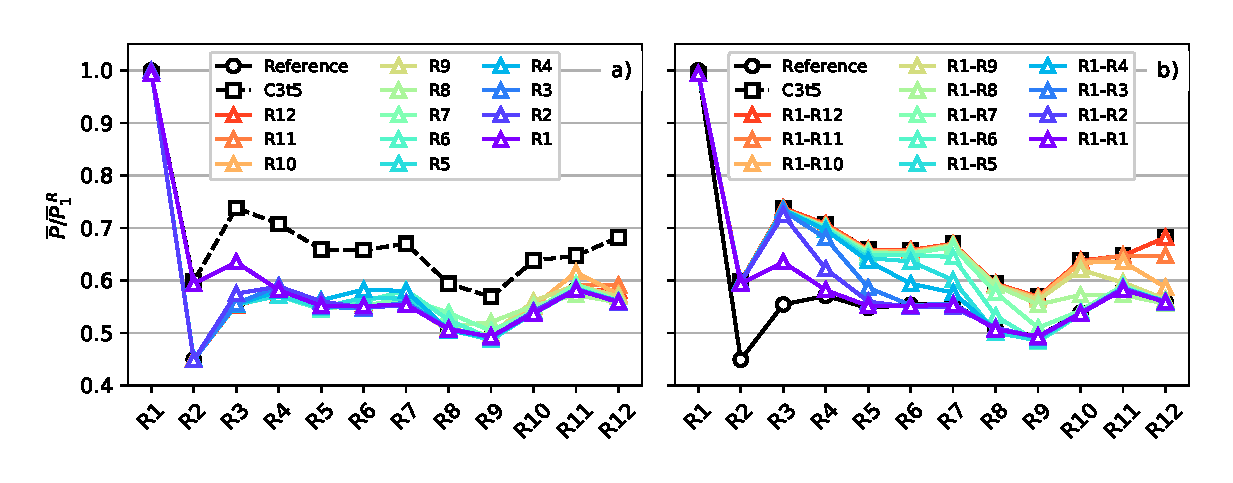
\includegraphics[width=\textwidth]{multirow.eps}
	\caption{Normalized row-averaged power extraction for the reference case, optimal control case C3t5, and subset control cases up to optimization window 3. \emph{a)} Subset control cases with optimal controls applied \emph{only} in one specific row. \emph{b)} Subset control cases with optimal controls applied \emph{for all rows up to} specific row. \label{fig:multirow}}
\end{figure}

\subsection{Optimization of single active turbine rows}\label{sec:optimization_single}
The previous section has shown that, based on the full-farm optimization case, the first-row controls can be applied independently, whereas this does not work for the downstream rows. To further quantify the potential for increasing wind-farm power in each row of turbines, the current section considers a set of additional optimal control cases in which \emph{only a single active row is optimized}, with all other rows remaining passive. Furthermore, by comparing the optimized controls of these cases with the full-farm optimization case C3t5, the degree of cooperation between turbines can be assessed. Note that the current single-row optimal control is not equivalent to greedy control: the optimizer still aims to increase aggregate farm power by taking into account wake interactions with downstream turbines. Furthermore, in contrast to the single-row control simulations from the previous section (i.e. in Figure~\ref{fig:multirow}a), the current optimizations will yield controls that are \emph{explicitly designed} to increase power given that all other rows are passive. To limit computational costs, the additional optimizations are only performed for a single time window. 

Figure~\ref{fig:single_row_opt} illustrates the relative increase in wind-farm power extraction for each of the twelve individually optimized control cases. The optimization is run until the continuous adjoint gradient accuracy prevents further progress in the vicinity of a local minimum (see discussion accompanying Figure~\ref{fig:window_opt}). Upon interpreting the actual values from the figure, it is important to note that the reported power gain covers the full optimization horizon $T$, and is hence affected by finite-horizon effects. Furthermore, the first window of an optimal control simulation, as considered here, contains an initial dead zone corresponding to the wake advection lag before upstream turbines start influencing their downstream neighbors. This tends to reduce gains compared to later time windows. Nevertheless, the relative order of the different cases still provides information that can be generalized to full optimal control studies with multiple windows and longer time horizons. 

The figure shows that the first row (R1) holds by far the most promise for optimizing wind-farm power. This is not surprising as R1 produces the most power of all rows, and typically leaves the deepest wakes, causing second-row turbines to perform  poorly in aligned wind-farm layouts (see, e.g., \citealp{porte2013numerical,nilsson2015large}; and \citealp{stevens2016effects}). At the other end of the spectrum, the last row (R12) is the least fruitful: it can only increase power by increasing $\cthat$ to harness the imperfections in the ADM for the given spatial resolution illustrated in Figure~\ref{fig:ct_sweep} (see discussion in Section~\ref{sec:analysis_thrust}), or by exploiting finite-horizon effects in which it attempts to completely halt the flow near the end of the time horizon. The intermediate rows (R2--R11) lie closer together, with the general trend being that potential is somewhat decreased with downstream distance into the wind farm, although this decrease is not monotonous. 

\begin{figure}
	\centering
	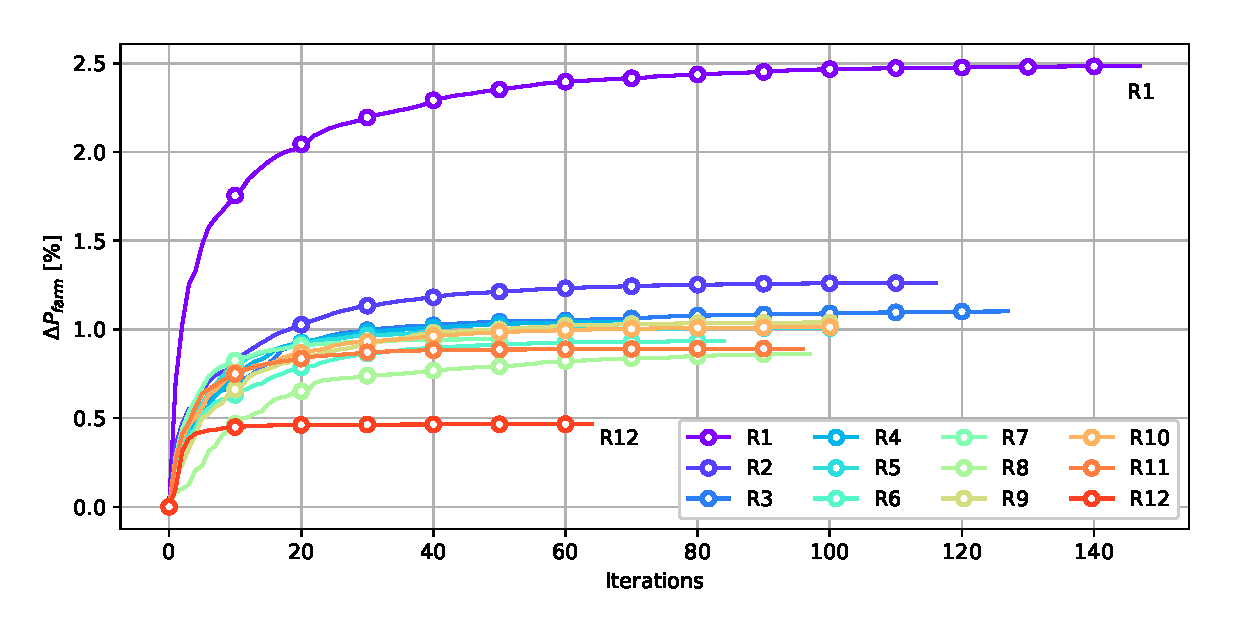
\includegraphics[width=\textwidth]{single_row_opt.eps}
	\caption{Increase in wind-farm power extraction for the first (and only) timewindow of the optimal control cases in which only a single row is optimized. \label{fig:single_row_opt}}
\end{figure}

Figure~\ref{fig:gains_singlerow} illustrates the row-wise relative power increase matrix for each of the single-row optimization cases. The figure indicates that, for each of the optimization cases, the largest power increase is observed in the first row downstream of the active turbine (i.e. R$_{\rm i+1}$), and that the influence on row R$_{\rm i+3}$ is limited. This is explained by the fact that the finite optimization horizon $T = 240$ s allows for more interactions with directly neighboring turbines than with those located further downstream. Furthermore, except for the optimal control case of the last row (R12), self-optimization is virtually non-existent: power gains are achieved by modifying the flow to yield more favorable conditions in the downstream rows. 

\begin{figure}
	\centering
	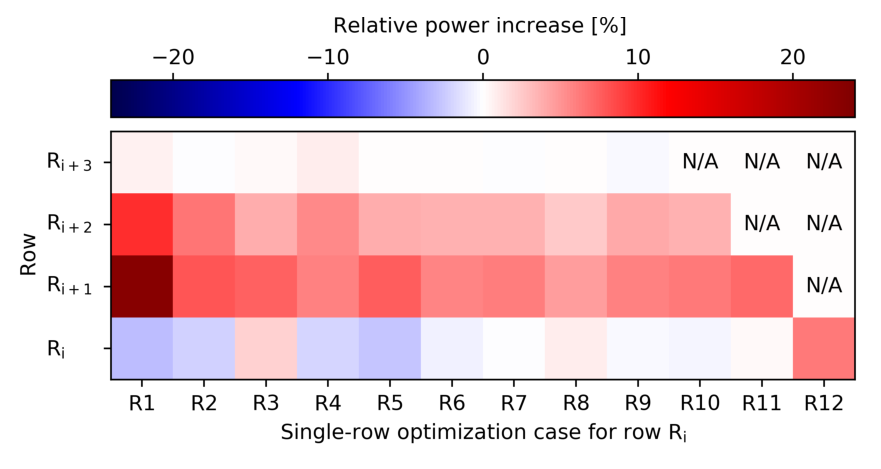
\includegraphics[width=0.9\textwidth]{individual_gains.eps}
	\caption{Relative power increase matrix for downstream rows in the single-row optimization case for row R$_{\rm i}$, indicated in the horizontal axis. N/A indicates non-existing downstream rows. Finite-horizon effects are eliminated by only reporting power increase up until $t = T_A$ for the active row R$_i$. \label{fig:gains_singlerow}}
\end{figure}

Turning to the thrust dynamics, Figure~\ref{fig:control_C3t5_singlerow} shows the optimized thrust coefficients for the entire optimization horizon $T$ in several turbine rows for the single-row (gray) and full-farm (black) optimizations. Interestingly, the first-row thrust coefficient is virtually identical, regardless of whether downstream turbines are active or not. Although similarities can also be observed for the downstream rows, the correspondence is much weaker than in the first row. This can be explained by the fact that, in contrast to the first row, downstream turbines experience different local flow conditions based on whether the upstream turbines are active or not.

\begin{figure}
	\centering
	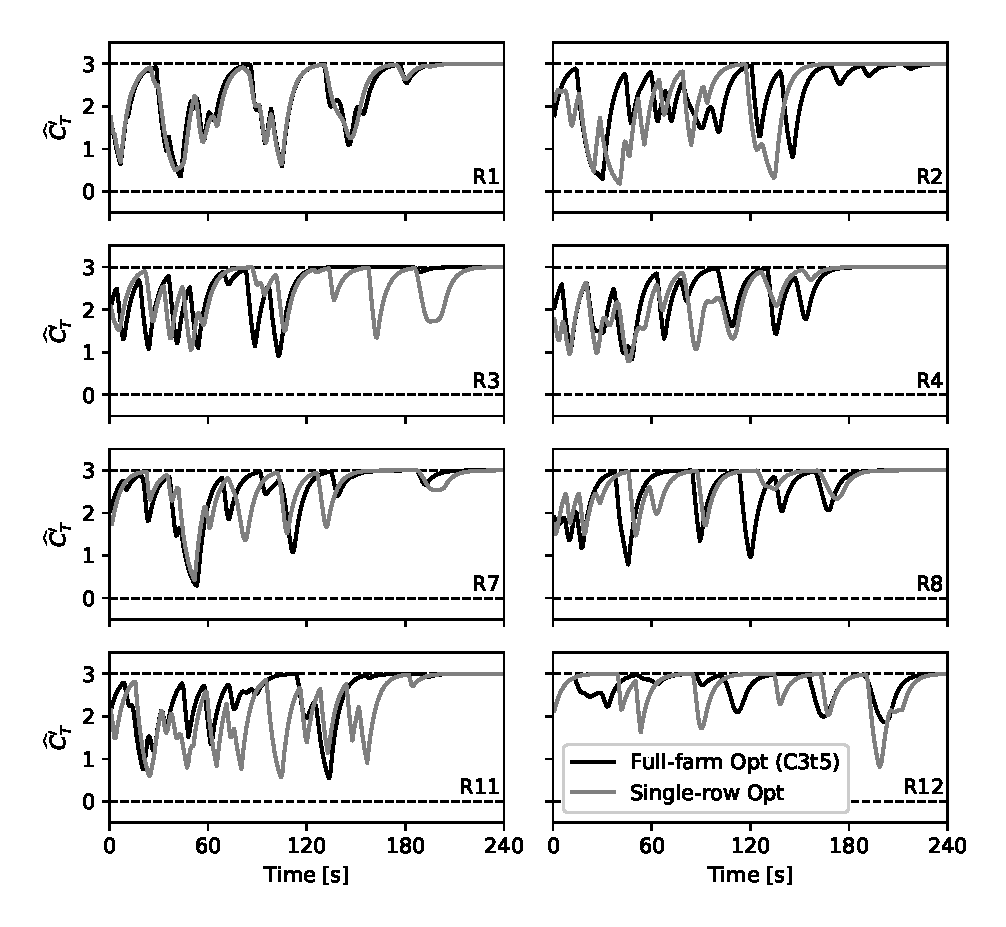
\includegraphics[width=0.9\textwidth]{fullfarm_singlerow.eps}
	\caption{Optimized thrust coefficients in several rows for case C3t5 (black) and single-row optimal control cases (gray) for the full optimization horizon $T = 240$ s.\label{fig:control_C3t5_singlerow}}
\end{figure}



The current observations further confirm the conclusions from previous section: optimal control actions depend to some degree on the local flow conditions. Furthermore, previous section showed that first-row controls still lead to power gains in the absence of downstream control response. Here, as indicated by the similarity in first-row controls for single-row and full-farm optimization cases, it is shown that, for the first row, the optimizer is actually indifferent to whether or not downstream rows are actively controlled. 


\subsection{Modification of thrust coefficient signals}\label{sec:modified_thrust}
The observations from previous sections illustrate that, at least to some degree, the optimized thrust coefficients are tuned to local flow conditions. In the current section, the possibility of whether the coefficients contain traits that are independent of flow conditions is nonetheless investigated. To this end, the optimized thrust coefficients are modified in such a way that correlations between them and specific flow events are eliminated. This is done in two independent test cases.

In the first case, the controls, which were specifically generated for selected turbines, are reassigned to other turbines by randomly swapping the control sets of different turbine columns. In doing so, each turbine will receive controls that were specifically designed for another turbine in the same row. To avoid erroneous conclusions based on coincidence, the column swap is performed in 2 random independent ways. Row-averaged power for these cases is shown in Figure~\ref{fig:scrambled}a. 

In the second case, controls remain assigned to their original turbines, but are shuffled in time by randomly swapping optimal controls generated for different control windows. In this way, the spectral thrust characteristics for timescales smaller that the control horizon $T_A = 120$ s remain unchanged, whereas the time synchronization of control actions to specific flow events is eliminated. Similar to the first case, this is done in 2 random ways, and Figure~\ref{fig:scrambled}b illustrates the row-averaged power for these cases.

The figure shows similar behavior for each of the modified control cases: only in the second row (R2), a consistent increase in power extraction can be observed. Combining this observation with the findings of previous sections, i.e. that power gains in a given row are caused by upstream control action instead of self-optimization, the current test cases suggest the presence of flow-invariant	features in the control signals of the first row. Note however that the full power gain in the second row is only partially attained, indicating that also the first turbine row reacts to the specific flow conditions. The small power increase in the last row (R12) can again be explained by the slightly higher mean value in $\cthat$. Based on the current data, no consistent gains in any of the other rows are found. 

\begin{figure}
	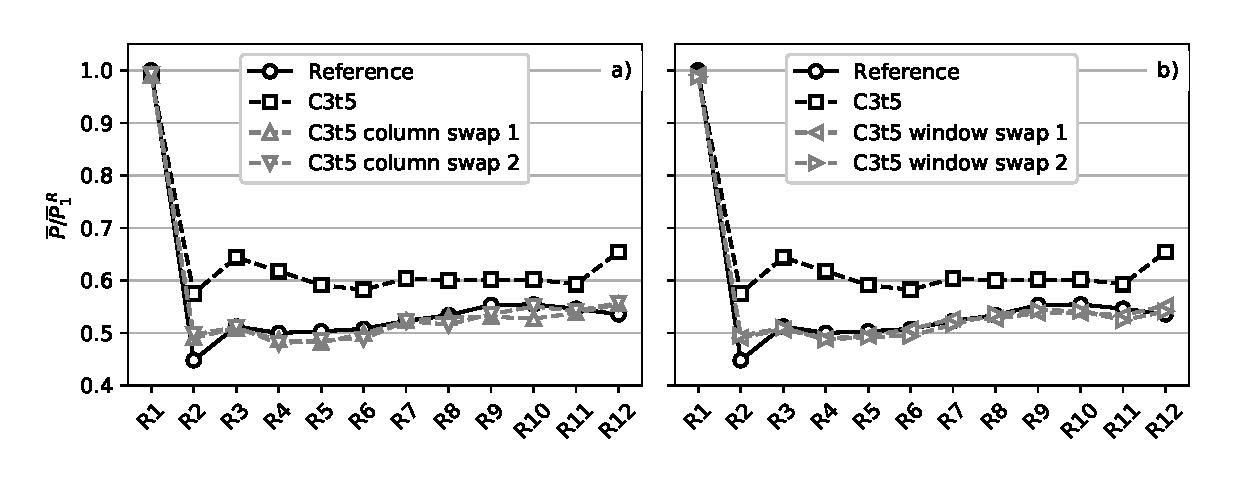
\includegraphics[width=\textwidth]{scrambled.eps}
	\caption{Normalized row-averaged power extraction for the reference case, optimal control case C3t5, and modified control cases. \emph{a)} Modified control cases with controls swapped between wind-turbine columns. \emph{b)} Modified control cases with controls swapped randomly by time window. \label{fig:scrambled}}
\end{figure}

\subsection{Discussion}\label{sec:analysis_discussion}

The observations and experiments from previous sections have revealed information that increases the understanding the optimized thrust coefficients, and can be used as a starting point towards designing practical wind-farm controllers that do not require computationally prohibitive LES-based optimal control simulations. A first conclusion that can be drawn from the analysis above is that wind turbines can be classified into three distinct categories, based on their position within the farm: first-row turbines, last-row turbines, and intermediate turbines.

The most salient behavior can be found in the first-row turbines (R1). Firstly, Figure~\ref{fig:spectra_thrust_cthat} showed that these turbines exhibit the largest variability in thrust coefficients and resulting thrust forces. Second, Figure~\ref{fig:multirow}a has shown that the optimized thrust coefficients in R1 are the only ones that can be applied independently from the other rows, and Figure~\ref{fig:single_row_opt} illustrated that the first row holds the greatest potential for power optimization of all rows in the farm. Third, the first row is the only one that has been shown to retain part of its power increase after eliminating the correlation between the optimized thrust coefficients and the flow field in Figure~\ref{fig:scrambled}, suggesting a flow-invariant component in the optimized coefficients. Finally, it is worth remarking the observed peak around $fD/U_\infty \approx 0.2 \dots 0.3$ from Figure~\ref{fig:spectra_thrust_cthat}. It will be shown below that variations in the thrust coefficient are related to specific flow events in the wake of R1.

The characteristics of the last row turbines (R12) also stand out from the rest. This is mainly caused by the fact that, by definition, the last row has no downstream turbines for which it can generate more favorable flow conditions, causing them to operate greedily in an optimal control setting. This explains the relatively quiescent behavior of optimized thrust coefficients in Figure~\ref{fig:controls}, and the limited potential for power increase in Figure~\ref{fig:single_row_opt}. 

The remaining intermediate rows (R2--R11) have similar spectral thrust characteristics (Figure~\ref{fig:spectra_thrust_cthat}) and potential for power increase (Figure~\ref{fig:single_row_opt}), situated in between but clearly separated from first- and last-row turbines. Further, it is worth noting that the behavior and analysis of control actions in these turbines is most complex: not only do they influence downstream turbines, they in turn are dependent on controls of upstream turbines. 

A second conclusion is that, whether or not the wind-farm is controlled with the possibility of active response and cooperation between turbines, the resulting power and thrust characteristics are very similar. Firstly, both Figure~\ref{fig:multirow}b (full-farm optimization) and Figure~\ref{fig:gains_singlerow} (single-row optimization) suggest that self-optimization of turbines is negligible, and that power gains are mainly achieved by generating more favorable flow conditions for downstream turbines. Furthermore, the remarkable match between optimized thrust coefficients for full-farm and single-row optimal control cases from Figure~\ref{fig:control_C3t5_singlerow} indicates that, at least for the first row, upstream controls do not rely on active downstream repose Instead, Figure~\ref{fig:multirow}b shows that, for any row $i$, the full potential in power increase is virtually attained by applying controls only for the upstream turbines up until row $i-1$. Furthermore, Figure~\ref{fig:multirow}a shows that optimized thrust coefficients in downstream rows by themselves do not result in power increase without also applying optimized coefficients in their upstream neighbors. This indicates that controls are tuned to specific flow events. This also explains the discrepancies between full-farm and single-row optimized thrust coefficients for downstream rows in Figure~\ref{fig:control_C3t5_singlerow}. 
These observations strongly suggest that the optimized thrust coefficients are designed in a parabolic manner, i.e. with a unidirectional propagation of control information from the first row to the last, and very little upstream influence of downstream turbine actions.

With this in mind, the remainder of this paper will focus on the first and most promising link of the control chain: the turbines situated in the first row of the wind farm.

\section{Flow visualization and mimicry of first-row behavior}\label{sec:analysis_flow_vis}
As shown in the previous section, the behavior of turbines within the first upstream row stands out from the others. Firstly, they are not influenced by any dynamic actions of the upstream turbines which makes their behavior somewhat easier to study. Secondly, they are unwaked and hence subjected to completely different flow characteristics than their downstream counterparts leading to much larger power extraction in the first row than downstream. Third, it was shown that the first-row controls show some inherent characteristics that are not tuned to specific flow events, and hence hold promise for simple and universally applicable control strategies. Therefore, the current section further focuses on the analysis of the first row. 

First, a qualitative analysis of the instantaneous flow field is performed in Section~\ref{sec:opt_visualization}, resulting in the observation of vortex rings being shed from first-row turbines. Thereafter, this mechanisms is mimicked by imposing sinusoidally varying thrust coefficients in these turbines in Section~\ref{sec:opt_sinus}, with the aim of increasing power through similar mechanisms as in the computationally expensive optimal control cases.

\subsection{Flow field visualization}\label{sec:opt_visualization}
With the aim of visualizing instantaneous flow field differences between controlled and reference cases, Figure~\ref{fig:vorticity_windfarm} illustrates snapshots of the velocity field at t = 300 s for the reference case (left) and the optimal control case C3t5 (right). Figures~\ref{fig:vorticity_windfarm}a,b show isosurfaces of vorticity magnitude, colored by streamwise velocity $\widetilde{u}_x$. Further, volumes of very low streamwise velocity (at $\widetilde{u}_x < 4.5 $ m s$^{-1}$) are rendered in black. Figure~\ref{fig:vorticity_windfarm}a shows that, in the reference case, the first-row turbines shed relatively stable vortex sheets that demarcate the wake from the freestream flow. The sheets destabilize and break up as they are advected downstream, resulting in complex three-dimensional vortical structures. Furthermore, as also shown in Figure~\ref{fig:vorticity_windfarm}c, wake mixing is limited, and downstream turbines experience reduced velocities. In contrast, the optimized case shows coherent vortex rings being shed from the first-row turbine. As indicated in Figure~\ref{fig:vorticity_windfarm}b, the locations of the rings in the controlled case coincide with naturally occurring bulges in the vortex sheet of the reference case: the controlled turbines further destabilize the sheet by well-timed temporal variations in its thrust coefficient. As illustrated in Figure~\ref{fig:vorticity_windfarm}c, this results in smaller velocity deficits in the wake region. Note that, downstream of the second turbine, the vorticity field becomes much more complex and differences in the flow fields are less coherent. 

The observed shedding of ring vortices seems to occur at specific flow-synchronized times to exploit natural instabilities in the original vortex sheets. Therefore, the remainder of this paper will attempt to accomplish the same effect by simple sinusoidal thrust variations. 

\begin{figure}
	\centering
	\includegraphics[width=\textwidth]{vorticity.eps}
	\caption{Instantaneous snapshots at t = 300 s of portion of wind-farm flow field for the reference (left) and optimized (right) case. \emph{a,b) } Isosurface of vorticity magnitude, colored by streamwise velocity $\widetilde{u}_x$. Deep wake regions (with $\widetilde{u}_x < 4.5$ m s$^{-1}$) are rendered in black. \emph{c)} Contours of streamwise velocity $\widetilde{u}_x$. Coloring is in units of m s$^{-1}$. Wind turbines are represented as gray disks. \label{fig:vorticity_windfarm}}
\end{figure}


\subsection{Sinusoidal thrust variations}\label{sec:opt_sinus}
The aim of the current section is to mimic the quasi-periodic shedding of vortex rings by upstream turbines as observed above through the use of simple periodic variations in the thrust coefficient. To this end, the Betz-optimal coefficient $\cthat = 2$ is perturbed by a sinusoidal signal, parametrized by its amplitude $A$, and a non-dimensional frequency in the form of the Strouhal number $St = f D/ U_\infty$:
\begin{equation}
\cthat(t) = 2 + A \sin \bigg(2\pi St \frac{t U_\infty}{D} \bigg).\label{eq:define_thrust}
\end{equation}

\subsubsection{Parameter sweep}
A parameter sweep is performed for both $A$ and $St$ on a reduced-size wind-farm LES, as illustrated in Figure~\ref{fig:sinus_setup}. The farm consists of $4 \times 4$ turbines in an aligned layout with $S = 6D$ in both streamwise and spanwise directions, geometrically equivalent to the optimally controlled wind farm from Chapter~\ref{ch:opt_induction}. The simulation is performed on a domain of $4 \times 2.4 \times 1$ km$^3$ with a simulation grid of $192 \times 256 \times 144$ gridpoints. Inflow conditions differ from those applied in the aforementioned simulations, and are generated by running an auxiliary shifted-periodic precursor simulation on a domain identical to the main simulation domain. All other simulation setup parameters are the same as those defined in Chapter~\ref{ch:opt_induction}. A set of wind-farm flow simulations is advanced in time by 30 minutes, during which the front row is controlled using a sinusoidally varying thrust coefficient $\cthat$, as defined in Equation \eqref{eq:define_thrust}. Within this set, the amplitude $A$ is varied between 0.5 and 2, with increments of 0.5. Furthermore, the Strouhal number $St$ is ranged between 0.05 and 0.6, with increments of 0.05. In total, this leads to 48 LES cases within the set. 

\begin{figure}
	\centering
	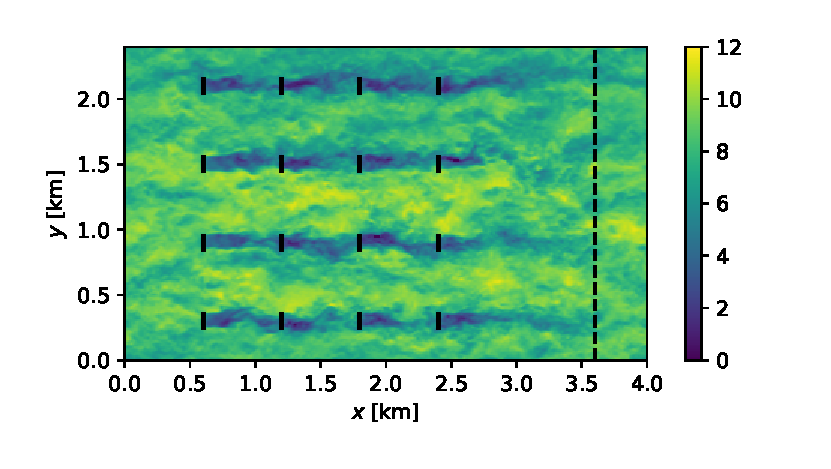
\includegraphics[width=0.75\textwidth]{setup_sinusoidal.eps}
	\caption{Reduced $4 \times 4$ wind-farm simulation setup for sinusoidal variation parameter study showing instantaneous contours of streamwise velocity $\widetilde{u}_x$. Coloring is in units of m s$^{-1}$. The dashed line indicates the start of the fringe region for imposition of unwaked inflow conditions. \label{fig:sinus_setup}}
\end{figure}

Figure~\ref{fig:sinus_baseline} illustrates the power extraction for all cases considered. Figure~\ref{fig:sinus_baseline}a illustrates the relative power gains over the reference case. From the figure it can be seen that there is a well-defined range of values for $A$ and $St$ for which wind-farm power can be increased substantially through upstream sinusoidal thrust variations, with a maximal power increase of $\approx$ 5\% at $(St^\star, A^\star) = (0.25, 1.5)$. In order to put the technical feasibility of these parameters into context, note that a Strouhal number $St = 0.25$ corresponds here to a sine wave period of $\approx$ 50 s for a turbine with diameter $D = 100$ m and a freestream velocity $U_\infty = 8.5$ m s$^{-1}$. The resulting maximum thrust coefficient of 3.5 could e.g. be attained by an NREL 5MW rotor with a 50\% increase in chord length (see \cite{goit2015optimal}, Appendix A). Figure~\ref{fig:sinus_baseline}b illustrates normalized power extraction by row for the reference case, the best sinusoidal case, and the first four rows of the optimal control case C3t5 from MM17. The figure shows that the power gain in the sinusoidal cases originates mostly from the second row, and that power in the first row is decreased by approximately 5\%. In contrast, optimal control case C3t5, in which all rows are active, also increases power in rows 3 and 4, and reduces first-row power by only 1\%. 
\begin{figure}
	\centering
	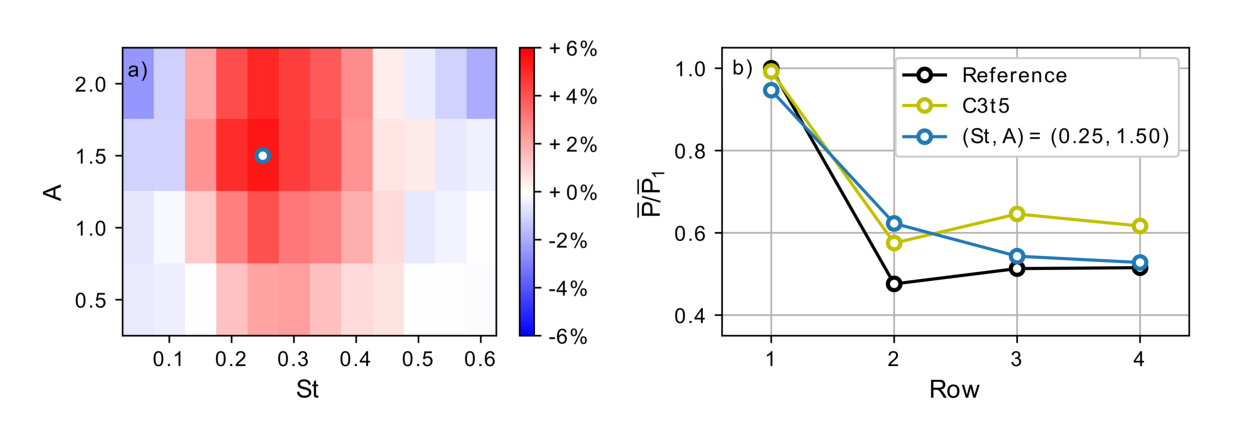
\includegraphics[width=\textwidth]{gains_turbulent_6D_6D_6D_wide_inphase2.eps}
	\caption{Power extraction of baseline sinusoidal thrust case ($S = 6D$, $z_0/H = 10^{-4}$). \emph{a) } Relative gain in mean wind-farm power extraction over reference case as a function of sine amplitude $A$ and frequency $St$. \emph{b) } Row-averaged mean power extraction for the best sinusoidal case, the optimal control case C3t5 from Chapter~\ref{ch:opt_induction}, and the reference case, normalized by first-row reference power.\label{fig:sinus_baseline} }
\end{figure}

Figure~\ref{fig:vorticity_parametersweep} illustrates instantaneous vorticity and axial velocities for a set of wind turbines of the aforementioned reference case (a), the best sinusoidal case with $(St, A) = (St^\star, A^\star)= (0.25, 1.5)$ (b), and a sinusoidal case which does not lead to increased power extraction with $(St, A) = (0.6, 2)$ (c). The figure illustrates that sinusoidal variations in the first-row thrust coefficient indeed cause periodic shedding of vortex rings. Figure~\ref{fig:vorticity_parametersweep}b shows that, at the optimal frequency, this leads to increased wake mixing, providing the second-row turbine with a higher incoming velocity. In contrast, Figure~\ref{fig:vorticity_parametersweep}c shows that, even though higher frequency thrust oscillations also result in periodic shedding of vortex rings, this does not automatically lead to more favorable flow conditions for downstream turbines. 
\begin{figure}
	\centering
	\includegraphics[width=\textwidth]{pumpcases2.eps}
	\caption{Snapshots of wind-farm flow fields at t = 1 800 s. \emph{Left: } Isocontours of vorticity, colored by streamwise velocity. \emph{Right: } Contours of streamwise velocity. \emph{a)} Reference. \emph{b)} Best sinusoidal case, with $(St , A) = (St^\star, A^\star) = (0.25, 1.5)$. \emph{c)} Sinusoidal case with $(St, A) = (0.6, 2)$ \label{fig:vorticity_parametersweep}  }
\end{figure}

In order to assess whether the same strategy can be used in the downstream turbines as well, Figure~\ref{fig:sinus_row2} illustrates the results from an identical parameter sweep as discussed above, except that here the second turbine row is controlled using a sinusoidal thrust coefficient. Figure~\ref{fig:sinus_row2}a indicates that sinusoidal actuation of the second row invariably leads to losses in wind-farm power. Figure ~\ref{fig:sinus_row2}b  shows that, for the optimal combination of parameters of  $(St, A) = (0.25, 1.5)$ as reported for first-row actuation above, the minor power increase in the third row does not compensate for additional losses in the second and fourth row. This shows that the proposed simple control strategy does not work when applied to waked turbines, and that more elaborate control strategies are required to harness the gains achieved by the optimal control simulation in the downstream regions of the farm. 
\begin{figure}
	\centering
	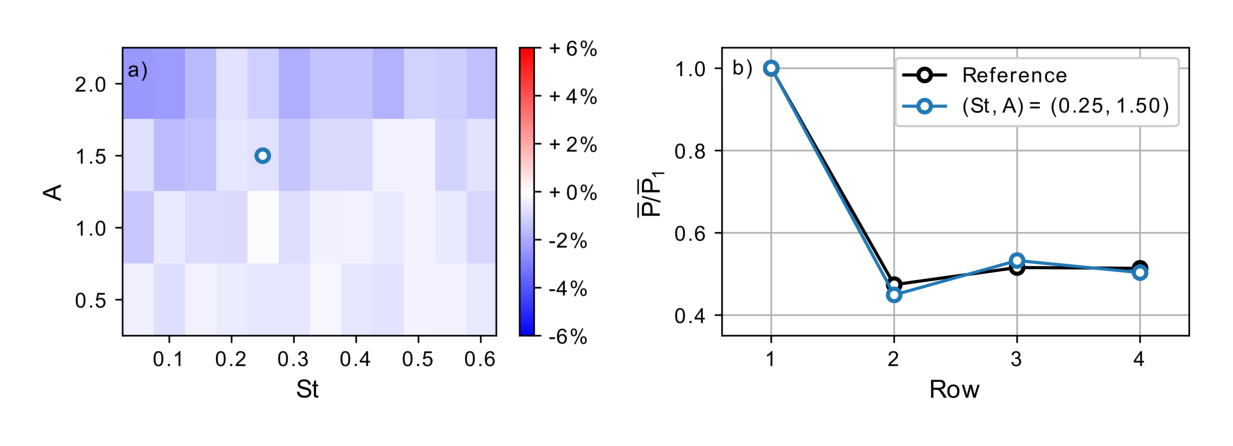
\includegraphics[width=\textwidth]{gains_row22.eps}
	\caption{Power extraction of second-row sinusoidal thrust case . \emph{a) } Relative gain in mean wind-farm power extraction over reference case as a function of sine amplitude $A$ and frequency $St$. \emph{b) } Row-averaged mean power extraction for the sinusoidal case with the optimal parameters as for row 1 sinusoidal thrust, and the reference case, normalized by first-row reference power.\label{fig:sinus_row2} }
\end{figure}

It is interesting to note that, even though the current parameter sweep is performed using different initial and inlet conditions, the optimal frequency of sinusoidal variations in $\cthat$ at $St^\star = f D / U_\infty = 0.25$ corresponds to the location of the peak in the first-row thrust coefficient spectrum in Figure~\ref{fig:spectra_thrust_cthat}. This suggests that the current vortex-shedding mechanism is related to the flow-invariant characteristics for increasing power reported in Figure~\ref{fig:scrambled}. 
In the following paragraphs, the robustness of the best parameter pair for first-row thrust variations, i.e. $(St, A) = (0.25, 1.5)$, is investigated with the aim of assessing the general applicability of this control strategy. To this end, similar parameter sweeps are performed for cases with varying turbine spacings and turbulence intensities.


\subsubsection{Robustness with respect to turbine spacing and turbulence intensity}

Figure~\ref{fig:sinus_spacing} illustrates the power extraction resulting from two parameter sweeps with streamwise turbine spacings of $5D$ and $7D$ respectively. Results are promising: for the given cases, $St^\star$ and $A^\star$  do not depend on streamwise turbine spacing. Furthermore, even in the $7D$ spacing case (Figure~\ref{fig:sinus_spacing}c-d), which naturally features lower overall power losses in downstream rows, power extraction in the second row can be significantly increased through sinusoidal variations in the first-row thrust coefficient. 
\begin{figure}
	\centering
	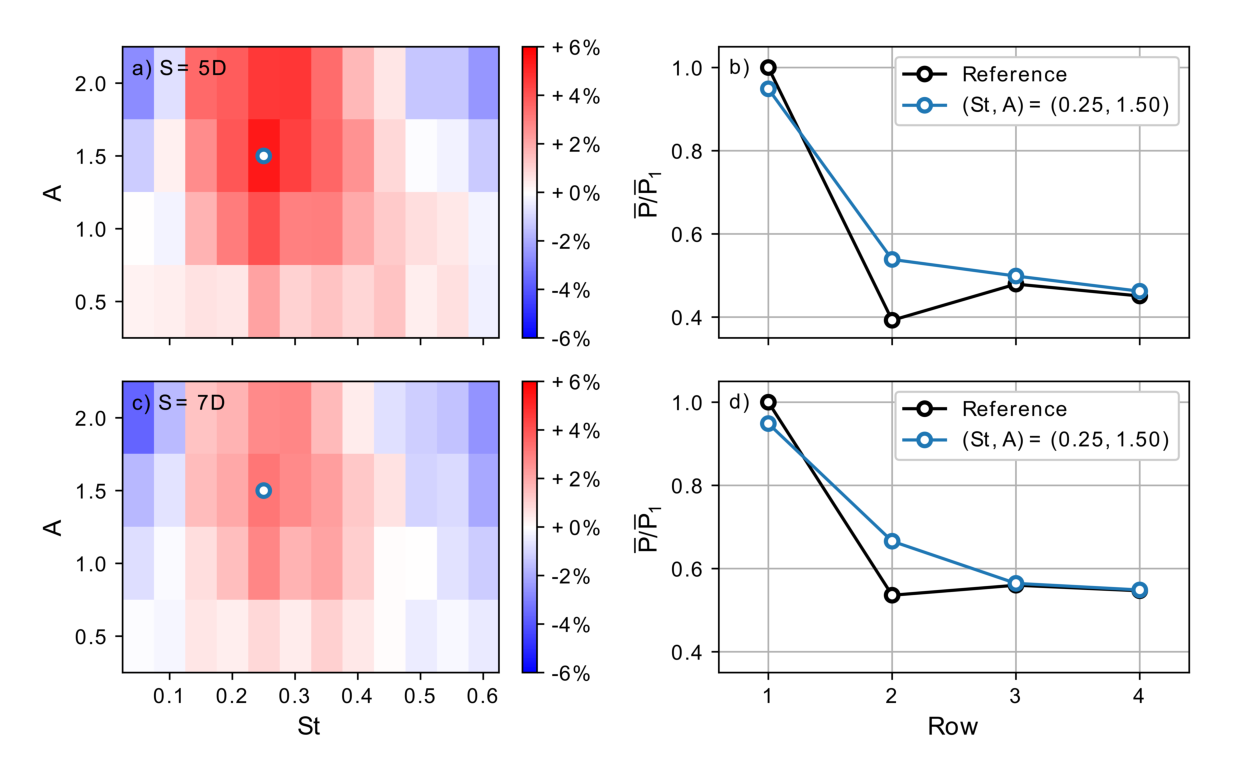
\includegraphics[width=\textwidth]{gains_combined2.eps}
	\caption{Power extraction of sinusoidal thrust cases with varying streamwise spacing. \emph{Top} (\emph{a,b}): Decreased spacing at $S = 5D$. \emph{Bottom} (\emph{c,d}): Increased spacing at $S = 7D$.  \emph{Left} (\emph{a,c}): Relative gain in mean wind-farm power extraction over reference case as a function of sine amplitude $A$ and frequency $St$. \emph{Right} (\emph{b,d}): Row-averaged mean power extraction for the best sinusoidal case and the reference case, normalized by first-row reference power. \label{fig:sinus_spacing} }
\end{figure}

Figure~\ref{fig:sinus_roughness} depicts the power extraction results from a parameter sweep with the same wind-farm layout as in the baseline case, but with a tenfold increase in roughness length, i.e. $z_0 = 10^{-3}H$. This results in a turbulence intensity of $\approx$ 16\%, compared to $\approx$ 10\% in the baseline case. Again, the best parameter combination of $(St^\star, A^\star) = (0.25, 1.5)$ remains unchanged. Further, even for this higher turbulence case, in which downstream losses are lower due to naturally better wake mixing, power is significantly increased in the second row, leading to a relative gain in wind-farm power of around 2\%. 
\begin{figure}
	\centering
	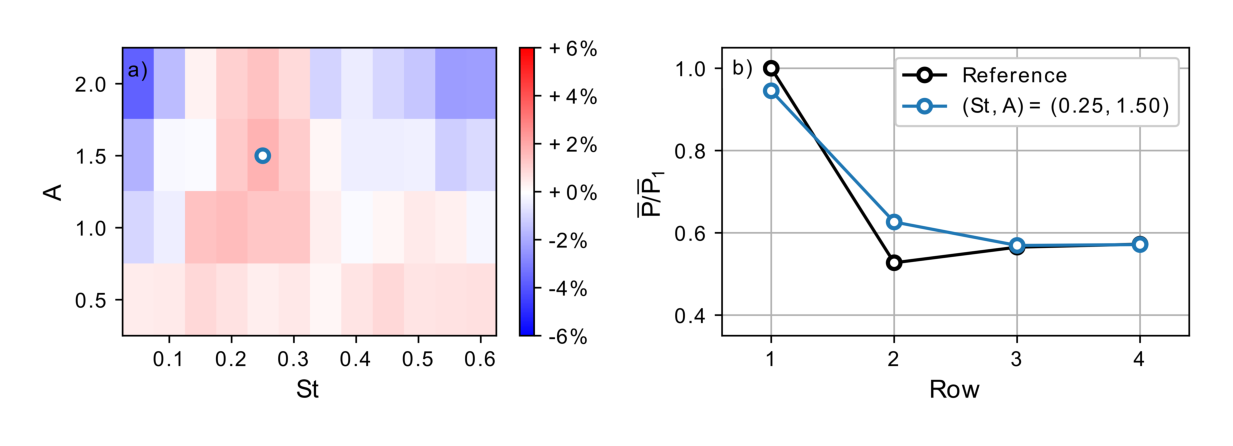
\includegraphics[width=\textwidth]{gains_turbulent_6D_6D_6D_wide_antiphase_z0_1m2.eps}
	\caption{Power extraction of sinusoidal thrust case with increased wall roughness $z_0/H = 10^{-3}$. \emph{a) } Relative gain in mean wind-farm power extraction over reference case as a function of sine amplitude $A$ and frequency $St$. \emph{b) } Row-averaged mean power extraction for the best sinusoidal case and the reference case, normalized by first-row reference power.\label{fig:sinus_roughness} }
\end{figure}

%\begin{figure}
%	\centering
%	\includegraphics[width=\textwidth]{pump.eps}
%	\caption{a = reference, b = row 1, c= row 2\label{fig:vorticity_pump}}
%\end{figure}

As evidenced above, periodic sinusoidal variations of first-row thrust coefficients substantially increase power extraction in the second row, resulting in a net gain in total power for the considered $4\times4$ wind farm. Moreover, different simulation sets indicate that, at least for the range considered here, the best values for Strouhal number and amplitude of these variations, i.e. $(St^\star, A^\star) = (0.25, 1.5)$, are robust with respect to turbine spacing and turbulence intensity. 

\subsubsection{Full-scale wind-farm test}
In the remainder of this section, the sinusoidal variation strategy will be tested in a full-scale wind farm, corresponding to the $12 \times 6$ aligned wind farm of Chapter~\ref{ch:opt_induction}. Simulations are performed for a reduced range of amplitudes and Strouhal numbers, corresponding to the most favorable region identified in the parameter sweeps above. In order to increase statistical convergence, the time horizon for each simulation is extended to a physical time of 10 hours. 

Figure~\ref{fig:sinus_fullscale} shows the power extraction of the full-scale test. Figure~\ref{fig:sinus_fullscale}a and~\ref{fig:sinus_fullscale}b show the relative power gains over the reference case for the full wind farm and the first four turbine rows respectively. A first observation is that the optimal pair $(St^\star, A^\star)$ differs for both measures, suggesting that the increased power in front rows entails losses in the downstream. This is confirmed by the row-wise power shown in Figure~\ref{fig:sinus_fullscale}c: from the fifth row onwards, power is slightly reduced in the sinusoidal cases. This explains the negligible increase in total farm power observed in Figure~\ref{fig:sinus_fullscale}a. 

\begin{figure}
	\centering
	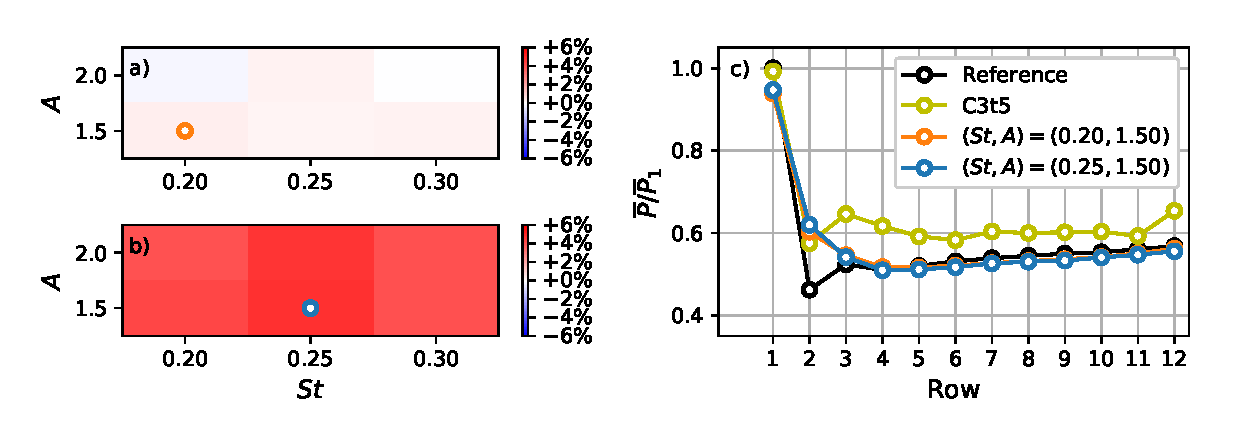
\includegraphics[width=\textwidth]{gains_fullscale.eps}
	\caption{Power extraction of full-scale sinusoidal thrust case ($S = 6D$, $z_0/H = 10^{-4}$). \emph{a) } Relative gain in mean wind-farm power extraction over reference case as a function of sine amplitude $A$ and frequency $St$. \emph{b) } relative gain in mean power extraction for the first four rows. \emph{c) } Row-averaged mean power extraction for the best sinusoidal case, the optimal control case C3t5 from Chapter~\ref{ch:opt_induction}, and the reference case, normalized by first-row reference power.\label{fig:sinus_fullscale} }
\end{figure}

The top panel of Figure~\ref{fig:cross_section_sinus} shows cross sections of time-averaged axial velocities $\widetilde{U}_x$ at the rotor disk locations for the reference case. Further, the middle and bottom panel illustrate deviations from the reference velocity for the $(St^\star, A^\star)$ sinusoidal case and the optimal control case C3t5 respectively.  The figure shows that both controlled cases show similar characteristics at the second turbine row, with an increased axial velocity at the rotor disk, accompanied by decreased velocities above and below. Downstream, it can be seen that the passive turbines of the sinusoidal case fail to retain increased velocities at the rotor disks, instead resulting in slightly lower disk velocities starting from the fifth row. In contrast, case C3t5, in which all turbines are actively controlled, succeeds to attain similar cross section characteristics with higher rotor velocities in the downstream as well. 

The current strategy hence succeeds in increasing total farm power for relatively short sets of aligned wind turbines. In contrast, larger wind farms require activity in downstream turbines as well to achieve significant gains in power extraction. However, it was found that the simple sinusoidal control strategy cannot be used in the intermediate rows. They are further discussed below in Section~\ref{sec:analysis_intermediate}

\begin{figure}
	\centering
	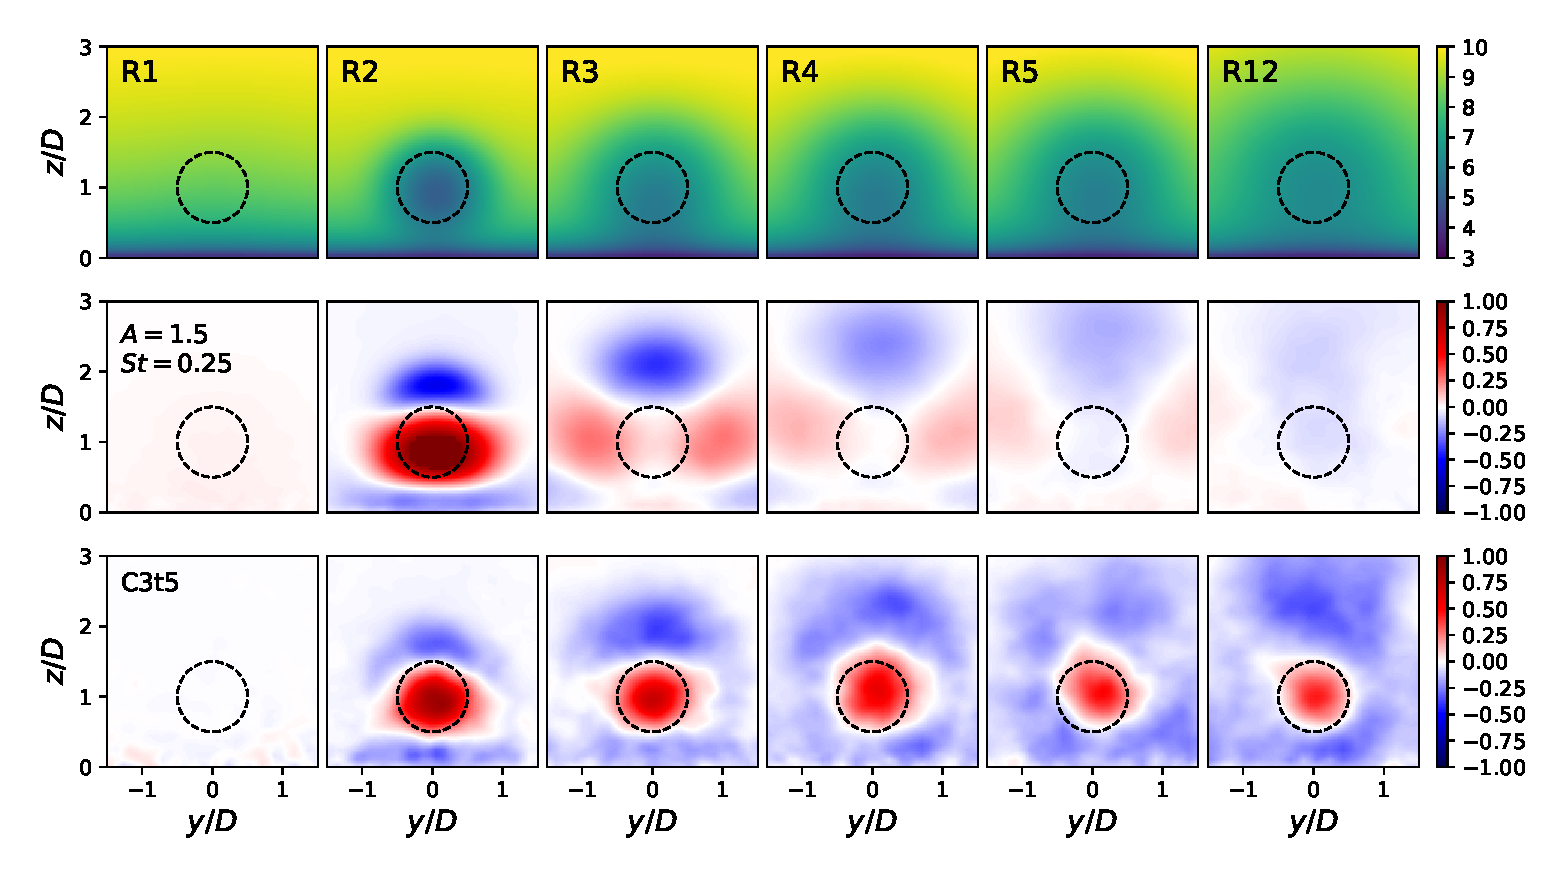
\includegraphics[width=\textwidth]{frontviews_allc3t5.eps}
	\caption{Cross section of time-averaged axial velocity $\widetilde{U}_x$ at rotor locations in rows 1, 2, 3, 4, 5, and 12. \emph{Top: } Reference case. \emph{Middle: } Difference between best sinusoidal perturbation case (with $A = 1.5$, $St = 0.25$) and reference case. \emph{Bottom: } Difference between optimal control case C3t5 and reference case. Coloring is in units of m s$^{-1}$. \label{fig:cross_section_sinus}}
\end{figure}

As shown throughout the current section, a qualitative analysis of instantaneous flow features in the optimal induction control wind farm from Chapter~\ref{ch:opt_induction} has led to the identification of a sinusoidal thrust control strategy for first-row turbines, resulting in increased power extraction in the second row. In contrast to earlier work on steady axial induction control, for which power gains have often been marginal or non-existent, the current analysis resulted in a robust axial induction control strategy with significant power gains, independent of specific local flow conditions. To the best knowledge of the author, this is the first time that optimal control simulations of wind farms are used to come up with simple control strategies, hence marking an important step towards practical dynamic axial induction control for increased power extraction. However, important comments should be made. First, sustained sinusoidal thrust variations with a large amplitude could contribute significantly to turbine fatigue loading. Hence, structural aspects should be taken into account upon evaluating the practical viability of the approach. Second, even though experiments have shown that, for practically relevant tip speed ratios, wind turbines shed vortices in a similar way as disk-like bluff bodies \citep{medici2006measurements}, the current behavior could still be an artifact of the relatively simple ADM used throughout this study. Further verification using higher fidelity wind turbine models, such as actuator line models, and wind-tunnel testing is hence necessary. 

\section{Intermediate-row behavior}\label{sec:analysis_intermediate}
The current section discusses the intermediate rows. It was shown that, without active participation in these rows, upstream gains are lost in downstream rows, and only full optimal control succeeds in achieving significant gains in downstream rows as well (see Figures~\ref{fig:sinus_fullscale},~\ref{fig:cross_section_sinus}). It was already mentioned that the analysis and behavior of turbines within intermediate rows is more complex than in the first row: they aim to influence the flow to the benefit of downstream rows but are also dependent on the actions of upstream rows. The remainder of the current section aims to illustrate the additional difficulty for power increase in downstream rows, and speculates on possible future paths for the identification of simplified control strategies as found for the first row.

First, as shown in the top panels of Figure~\ref{fig:cross_section_sinus}, even in the uncontrolled case, the kinetic energy of the flow in the vicinity of the turbine rotor is depleted more and more in the downstream rows. This complicates control strategies for these rows as the opportunity for increased mixing with high energy winds is decreased. Furthermore, intermediate turbines are subjected to increased turbulence levels and more complex vorticity dynamics, as illustrated in Figure~\ref{fig:vorticity_windfarm}. This could explain why the sinusoidal thrust control for the first row did not lead to increase power when applied to the second row: whereas the first row produces increased mixing by destabilizing relatively stable vortex sheets into vortex rings, the second row is already continuously immersed in complex vorticity patterns for which this simple approach does not work. 
However, note that for instance R7 in Figure~\ref{fig:controls} also seems to show quasi-periodic sinusoidal variations in $\cthat$ at a time period of approximately 50~s. This could be an indication that, also for intermediate rows, vortex ring shedding could amount to part of the power increase of observed in the optimal control simulations, albeit at specific moments in time, synchronized with the local flow conditions.

Second, it is important to note that the vortex ring shedding mechanism constitutes only part of the power increase caused by the first row. Figure~\ref{fig:multirow} illustrates that the first-row optimized thrust coefficient also results in a significant power increase in the third row, which is not observed using the sinusoidal thrust strategy. Furthermore, the analysis of the modified control cases in Figure~\ref{fig:scrambled} proves that also the first-row controls are partially synchronized with the flow. This shows that other mechanisms, dependent on specific flow events for increasing wind-farm power, are at play as well. Even though the application of regression algorithms in an attempt to link turbine actions to low-dimensional flow measurements (e.g. local velocity, shear and kinetic energy) has been unsuccessful thus far, similar analysis based upon more complex flow features (e.g. vorticity structures, high-speed turbulent streaks, or downdrafts) might be more promising. However, this requires further optimal control simulations over an extended time, as the total control time horizon of 30 minutes in the current dataset is expected to be insufficient for robust statistics in this kind of analysis. This is an important remaining challenge to be addressed in future research. 

%\section{Summary}\label{sec:analysis_summ}
\conclusions \label{sec:analysis_summ}
The current paper provided a further analysis of the thrust coefficient control characteristics for the C3t5 optimal control case from Chapter~\ref{ch:opt_induction}. 

Analysis of the thrust coefficients and numerical experiments have shown a clear distinction between first-row turbines, last-row turbines, and intermediate turbines. Furthermore, observations strongly suggest that the optimization works in a unidirectional way: upstream turbines influence the flow field resulting in favorable conditions for their downstream neighbors, yet information on the possibility of active response and cooperation in the latter has very little influence on upstream control actions. 

Qualitative analysis of instantaneous flow fields led to the observation of quasi-periodic shedding of vortex rings from first-row turbines in the optimal control case. This flow feature was succesfully mimicked using simple sinusoidal thrust actuation of the first row. The best parameter set for these sinusoidal variations proved robust to both wind-turbine spacing and turbulence intensity, with a non-dimensional frequency at $St^\star = 0.25$. Interestingly, this frequency corresponds to the peak at $St = 0.2 \dots 0.3$ observed in the first-row thrust coefficient spectra. Since the optimal value $St^\star$ was found using a different realization of the turbulent wind-farm flow, this indicates that the vortex-shedding mechanism is linked to the flow-invariant traits of the first-row optimal controls of case C3t5. Although the first-row sinusoidal control led to a robust increase in total power for a reduced-size $4\times4$ wind farm, a full-scale test indicated that downstream turbine activity is required to obtain increased power at larger farm scales. Further, it was shown that the simple sinusoidal strategy does not lead to increase power extraction when applied to downstream intermediate turbines. Identifying the mechanisms for power increase in these turbines hence remains an important open research question. 


\dataavailability{TEXT} %% use this section when having only data sets available

%\appendix
%\section{}    %% Appendix A
%\subsection{}     %% Appendix A1, A2, etc.
%\noappendix       %% use this to mark the end of the appendix section

\competinginterests{The authors declare no conflict of interest.} %% this section is mandatory even if you declare that no competing interests are present

\begin{acknowledgements}
The authors acknowledge funding by the European Research Council (grant no. 306471). The computational resources and services used in this work were provided by the VSC (Flemish Supercomputer Center), funded by the Research Foundation - Flanders (FWO) and the Flemish Government, department EWI.
\end{acknowledgements}




%% REFERENCES
%\begin{thebibliography}{}
%
%\bibitem[AUTHOR(YEAR)]{LABEL}
%REFERENCE 1
%
%\bibitem[AUTHOR(YEAR)]{LABEL}
%REFERENCE 2
%
%\end{thebibliography}


\bibliographystyle{copernicus}
\bibliography{bib_induction_energies}


%% LITERATURE CITATIONS
%%
%% command                        & example result
%% \citet{jones90}|               & Jones et al. (1990)
%% \citep{jones90}|               & (Jones et al., 1990)
%% \citep{jones90,jones93}|       & (Jones et al., 1990, 1993)
%% \citep[p.~32]{jones90}|        & (Jones et al., 1990, p.~32)
%% \citep[e.g.,][]{jones90}|      & (e.g., Jones et al., 1990)
%% \citep[e.g.,][p.~32]{jones90}| & (e.g., Jones et al., 1990, p.~32)
%% \citeauthor{jones90}|          & Jones et al.
%% \citeyear{jones90}|            & 1990

\end{document}
